\documentclass[a4paper,titlepage,11pt,floatssmall]{mwrep}
\usepackage[left=2.5cm,right=2.5cm,top=2.5cm,bottom=2.5cm]{geometry}
\usepackage[OT1]{fontenc}
\usepackage{polski}
\usepackage[utf8]{inputenc}
\usepackage{amsmath}
\usepackage{amsfonts}
\usepackage{amssymb}
\usepackage{graphicx}
\usepackage{url}
\usepackage{tikz}
\usetikzlibrary{arrows,calc,decorations.markings,math,arrows.meta}
\usepackage{rotating}
\usepackage[percent]{overpic}
%\usepackage[cp1250]{inputenc}
\usepackage{xcolor}
\usepackage{pgfplots}
\usetikzlibrary{pgfplots.groupplots}
\usepackage{listings}
\usepackage{matlab-prettifier}
\usepackage{siunitx}
\usepackage{placeins}
\definecolor{szary}{rgb}{0.95,0.95,0.95}
\sisetup{detect-weight,exponent-product=\cdot,output-decimal-marker={,},per-mode=symbol,binary-units=true,range-phrase={-},range-units=single}

\SendSettingsToPgf
\title{\bf Sprawozdanie z laboratorium nr 2 \\ Projekt licznika 4-bitowego przy użyciu procesora Zilog Z80 \vskip 0.1cm}
\author{Jakub Sikora \and Konrad Winnicki \and Marcin Dolicher}
\date{\today}
\pgfplotsset{compat=1.15}	
\begin{document}


\makeatletter
\renewcommand{\maketitle}{\begin{titlepage}
		\begin{center}{\LARGE {\bf
					Wydział Elektroniki i Technik Informacyjnych}}\\
			\vspace{0.4cm}
			{\LARGE {\bf Politechnika Warszawska}}\\
			\vspace{0.3cm}
		\end{center}
		\vspace{5cm}
		\begin{center}
			{\bf \LARGE Technika Mikroprocesorowa \vskip 0.1cm}
		\end{center}
		\vspace{1cm}
		\begin{center}
			{\bf \LARGE \@title}
		\end{center}
		\vspace{2cm}
		\begin{center}
			{\bf \Large \@author \par}
		\end{center}
		\vspace*{\stretch{6}}
		\begin{center}
			\bf{\large{Warszawa, \@date\vskip 0.1cm}}
		\end{center}
	\end{titlepage}
	}
\makeatother
\maketitle

\tableofcontents


% pierwsza sekcja
\chapter{Polecenia}

\section{Zadanie podstawowe}
\indent{} Celem drugiego zadania laboratoryjnego było zaprojektowanie, złożenie, zaprogramowanie i przetestowanie układu z procesorem ZILOG Z80 emulowanego w układzie FPGA tak aby działał on jako licznik 4-bitowy zliczający w dół liczbę wciśnięć programowo odszumionego przycisku monostabilnego, który umożliwiał asynchroniczne ładowanie liczby do pamięci z blokowaniem zliczania. Ładowanie liczby powinno odbyć się przy pomocy przerwania maskowalnego. Liczby powinny być przechowywane w Naturalnym Kodzie Binarnym, w skrócie NKB.

\section{Zadanie dodatkowe}
\indent{} W trakcie zajęć otrzymaliśmy również zadanie dodatkowe na podniesienie oceny. W ramach tego zadania mieliśmy zastanowić się czy możliwym jest zaprojektowanie systemu wielowątkowego na układzie z procesorem Z80 i opisanie jeśli to możliwe jak należy to zrobić lub jeśli nie jest to możliwe, opisać dlaczego.


\chapter{Projekt licznika}
\section{Opis rozwiązania}
\indent{} Pierwszym problemem z jakim przyszło nam się zmierzyć podczas opracowywania rozwiązania był projekt układu w którym procesor Z80 miał pracować. Musieliśmy wziąć pod uwagę cykle zapisu procesora do peryferiali oraz możliwość współpracy z układami wspierającymi. Ostatecznie zdecydowaliśmy się na skorzystanie układów 74HC541 oraz 74HC574, do poprawnej obsługi wejścia/wyjścia. W przypadku operacji zapisu do przestrzeni I/O, sygnały z przycisków były najpierw kierowane na matrycę buforów trójstanowych (układ 74HC541) aby w odpowiednim momencie gdy pojawi się kombinacja aktywnych sygnałów $\overline{IORQ}$ oraz $\overline{RD}$ mogły zostać one zapisane na szynę danych procesora i wpisane do odpowiedniego rejestru. \indent{} Analogicznie procesor zachowywał się podczas zapisu stanu licznika na układ ośmiu diod. Aby rezultat mógł zostać zauważony, musieliśmy dodać do diod układ pamiętający, którego rolę spełnił układ 74HC574 czyli matryca ośmiu przerzutników typu D. Układ aktywowany był sumą logiczną sygnałów $\overline{IORQ}$ oraz $\overline{WR}$ tak aby podczas zapisu do przestrzeni I/O układ zapamiętał stan szyny i podtrzymywał go na swoich wyjściach do momentu nadejścia kolejnego sygnału zapisu. 

\begin{figure}[th]
\centering
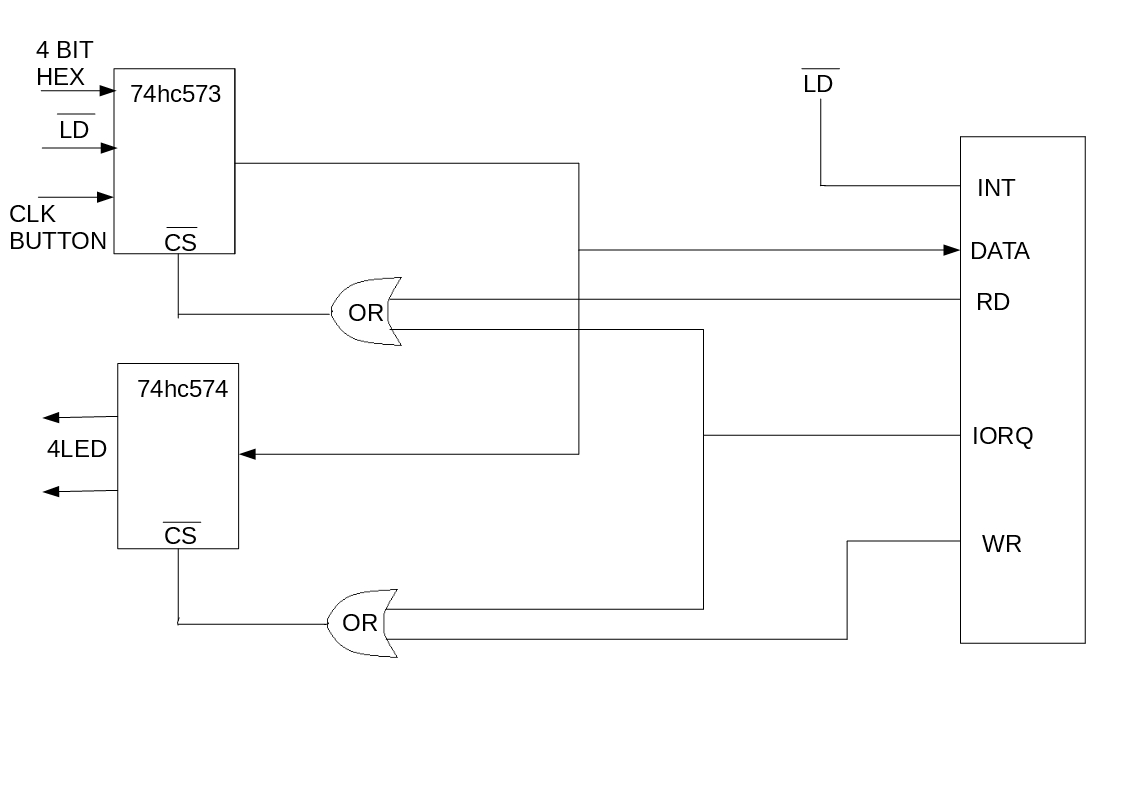
\includegraphics[width=\textwidth]{ideowy}
\caption{Schemat ideowy}
\end{figure}

\section{Oprogramowanie}

\indent{} Oprogramowanie procesora zostało przez nas napisane w asemblerze. Takie rozwiązanie wiązało się z poznaniem składni języka asemblera procesora Z80 oraz z ogólnymi zasadami pisania kodu niskopoziomowego. 
\subsection{Odszumianie przycisku}
\indent{} Docelowo procesor miał programowo odszumiać przycisk monostabilny. Styki takiego przycisku przy wciśnięciu zaczynają drgać, wielokrotnie zmieniając swój stan z wysokiego na niski. Kod sprawdzający zmianę stanu przycisku mógłby odczytać takie pojedyncze wciśnięcie jako kilka lub kilkadziesiąt wciśnięć. W celu poprawnego zliczania wciśnięć przycisku, w pętli głównej aplikacji zliczaliśmy 255 wystąpień stanu wskazującego na wciśnięcie. W przypadku pojawienia się odbicia styków, cały proces zliczania miał zostać  wyzerowany. Analogicznie, program miał wykrywać puszczenie przycisku tak aby był w stanie oddzielać od siebie dwa różne wciśnięcia przycisku. W programie nie występują pętle zliczające w umożliwienia poprawnej pracy innych programów na procesorze.
\subsection{Ładowanie do licznika}
\indent{} Zaprojektowany przez nas licznik ma również możliwość asynchronicznego ładowania. Została ona zrealizowana przy pomocy maskowalnego przerwania. Przerwanie jest obsługiwane w trybie IM1, dlatego też kod obsługi przerwania rozpoczyna się adresu 0x0038. W procedurze obsługi znajduje się kolejno wrzucenie zawartości rejestru AF na stos, wczytanie liczby do licznika z portu wejściowego, wybranie 4 najmłodszych pobranych bitów, załadowanie ich do rejestru zliczającego, odświeżenie diod i ostatecznie operacje powrotu z przerwania. 
\subsection{Sekcje krytyczne}
\indent{} Do programu musieliśmy wpleść sekcje krytyczne przy zmianie wartości którą przechowuje licznik. Sekcje krytyczną utworzyliśmy przy pomocy operacji DI oraz EI, które odpowiednio blokują i umożliwiają dalsze przyjecie przerwania. 

\subsection{Listing programu}
\begin{flushleft}
\#  File miracle.asm \\
0000			; Licznik 4-bit, kod NKB, ładowanie, zliczanie w dół\\
0000			; \\
0000			; Wykorzystanie rejestrów:  \\
0000			;	B - zawiera wartość licznka, \\ 
0000			;	C - licznik debounce,  \\
0000			;	D - ilość cykli debounce \\
0000			;	E - stan układu licznika, 1 dla obsługi zbocza narastającego, 0 dla obsługi zbocza opadającego; \\
0000			; \\
0000			; Podłączenie przycisków:  \\
0000			;	CLK - bit 6 \\
0000			;	!LD - bit 5 ( jednocześnie podłączony do !INT )\\ 
0000			;	DANE -bity <0..3> \\
0000			; \\
0000			org 1800h \\
1800			START: \\
1800 31 ff 1f			LD SP, 0x1FFF ; Ustawienie wskaźnika stosu \\
1803 18 5b			jr MAIN  \\
1805 0x00...		ds 0x1838-\$,0 ; Umieszczenie procedury przerwania pod adresem 0x38 \\
1838			INTERRUPT: 		; obsługa przerwania od przycisku !LD \\
1838 f5				PUSH AF 	; Zapisanie na stosie rejestrów A i F \\
1839 db 01			IN A, (1) 	; wczytanie danych do załadowania \\
183b e6 0f			AND 0Fh 	; wybranie istotnych danych \\
183d 47				LD B, A		; załadowanie licznika \\
183e d3 01			OUT (1), A	; odświeżenie LED \\
1840 f1				POP AF		; przywrócenie stosu i powrót z przerwania \\
1841 fb				EI \\
1842 c9				RET \\
1843 0x00...		ds 0x1860-\$,0 ;org 1860h \\
1860			MAIN: \\
1860 db 01			IN A, (1) 	; inicjacja wartości licznika \\
1862 e6 0f			AND 0Fh		; wybranie istotnych danych \\
1864 47				LD B, A		; wpisanie początkowej wartości do licznika \\
1865 d3 01			OUT (1), A	; odświeżenie licznika \\
1867 16 ff			LD D, 255 	; ilość cykli debounce \\
1869 ed 56			IM 1 \\
186b fb				EI	 \\
186c 4a				LD C, D 	; ustawienie licznika debounce \\
186d 1e 00			LD E, 0 	; wybrana obsługa zbocza opadającego \\
186f			MAIN\_LOOP: 		; początek głównej pętli \\
186f			 \\
186f				; początek obsługi licznika \\
186f 7b					LD A, E \\
1870 e6 ff				AND 0xFF	; odświeżenie stanu flag \\
1872 20 1b				JR NZ, LOOP\_POSITIVE ; wybranie obsługi konkretnego zbocza \\
1874				LOOP\_NEGATIVE:	; obsługa zbocza opadającego \\
1874 db 01				IN A, (1) \\
1876 cb 77				BIT 6, A 	; stan przycisku CLK \\
1878 28 01				JR Z, IF\_1 \\
187a 4a					LD C, D 	; jeśli przycisk niewciśnięty, załaduj licznik debounce \\
187b				IF\_1: \\
187b 20 01				JR NZ, IF\_2 \\
187d 0d					DEC C 		; jeśli przycisk wciśnięty, dekrementuj licznik debounce \\
187e				IF\_2: \\
187e 79					LD A, C		; odświeżenie stanu flag \\
187f e6 ff				AND 0xFF \\
1881 20 1d				JR NZ, COUNTER\_END ; jeśli licznik debounce niezerowy, koniec obsługi \\
1883 05					DEC B		; wykryto poprawne zbocze opadające, akcja licznika \\
1884 f3					DI			; sekcja krytyczna \\
1885 78					LD A, B		;  \\
1886 e6 0f				AND 0Fh \\
1888 d3 01				OUT (1), A	; odświeżenie LED \\
188a fb					EI			; koniec sekcji krytycznej \\
188b 1e 01				LD E, 1		; wybranie obsługi zbocza narastającego \\
188d 18 11				JR COUNTER\_END ; skok na koniec obsługi licznika \\
188f				LOOP\_POSITIVE:	; obsługa zbocza narastającego\\ 
188f db 01				IN A, (1) \\
1891 cb 77				BIT 6, A 	; stan przycisku CLK \\
1893 20 01				JR NZ, IF\_3 \\
1895 4a					LD C, D		; jeśli przycisk wciśnięty, załaduj licznik debounce \\
1896				IF\_3: \\
1896 28 01				JR Z, IF\_4 \\
1898 0d					DEC C		; jeśli przycisk niewciśnięty, dekrementuj licznik debounce \\
1899				IF\_4: \\
1899 79					LD A, C		; odświeżenie stanu flag \\
189a e6 ff				AND 0xFF \\
189c 20 02				JR NZ, COUNTER\_END ; jeśli licznik debounce niezerowy, koniec obsługi \\
189e 1e 00				LD E, 0 \\
18a0				COUNTER\_END:	; koniec obsługi licznika \\
18a0			 \\
18a0				; dalsze operacje...	 \\
18a0			 \\
18a0 18 cd		JR MAIN\_LOOP ; powrót do początku głównej pętli\\
\# End of file miracle.asm\\
18a2\\
\end{flushleft}


\chapter{System wielowątkowy}
\indent{} W ramach zadania dodatkowego mieliśmy zastanowić się i opisać czy możliwym jest w ramach układu z procesorem Z80 zrealizować system obsługujący 4 wątki.
\begin{center}
\textit{Czy w procesorze Z80 możliwe jest zaimplementowanie wielowątkowości?}\\
\end{center}
Naszym zdaniem jest to możliwe, co więcej, istnieją dwie metody na realizację tego zadania.\\\\
1.	Wielowątkowość bez wywłaszczania (bez wstrzymywania pracy wątków)
Realizacja polega na strukturze programu nadrzędnego(planisty) który w pętli wywołuje kolejno procedury wątków( bezpośrednio np. CALL WATEK\_01 lub może jakaś lista wątków), wątki zobligowane są do wykonania swoich zadań w możliwie najkrótszym czasie(bez blokowania CPU) i oddania sterowania do planisty(powrotu do miejsca wywołania, czyli np. RET)\\
Przykładowy pseudokod planisty: \\ \\
START:\\
Inicjacja CPU oraz sprzętu\\ 
MAIN:\\
CALL WATEK\_01\\
CALL WATEK\_02\\
CALL WATEK\_03\\
CALL WATEK\_04\\
JP MAIN: \\
\\
\\
2.  Wielowątkowość z wywłaszczaniem ( z możliwością wstrzymywania wątków)
Proponowana realizacja polega na zewnętrznym układzie generującym żądanie przerwania niemaskowalnego przykładowo co 100 taktów zegara lub co 100 wystąpień stanu niskiego na linii M1, co daje nam przydział około 100 instrukcji każdemu wątkowi, po czym następuje kolejne przerwanie i zmiana aktywnego wątku.
Wybór aktywnego wątku następuje w procedurze obsługi przerwania niemaskowalnego,  procedura zachowuje aktualną zawartość rejestrów przypisaną do wątku który właśnie stracił kontrolę nad CPU(zachowywany jest również adres powrotu), przywraca stan rejestrów powiązany z wątkiem który otrzymuje właśnie kontrolę, modyfikowany jest również adres powrotu z przerwania niemaskowalnego dzięki czemu po wywołaniu instrukcji powrotu wykonany zostanie skok do miejsca gdzie w przeszłości przerwany został wątek który otrzymał właśnie sterowanie nad CPU
Przykładowy pseudokod obsługi przerwania niemaskowalnego:\\
IF źródło==ext\_gen\_100 \\
LD (WATEK\_01\_MEM\_ADDR++), RETURN\_SP\\
LD (WATEK\_01\_MEM\_ADDR++), ABCDEFGH\\
LD ABCDEFGH, (WATEK\_02\_MEM\_ADDR--)\\
LD RETURN\_SP, (WATEK\_02\_MEM\_ADDR--)\\
RETN\\


\end{document}

\end{document}